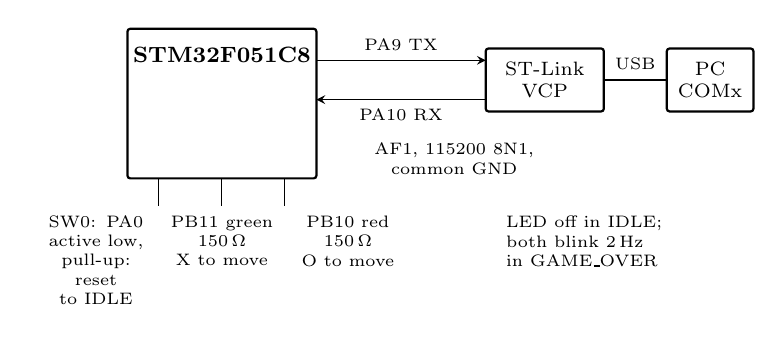
\begin{tikzpicture}[x=1cm,y=1cm,font=\scriptsize,
  box/.style={draw,thick,rounded corners=1pt,align=center,inner sep=2pt}]
 \node[box,minimum width=2.4cm,minimum height=1.9cm] (mcu) at (0,0) {};
 \node[font=\footnotesize\bfseries] at (0,0.62) {STM32F051C8};
 \node[box,minimum width=1.5cm,minimum height=0.8cm] (stl) at (4.1,0.3) {ST-Link\\VCP};
 \node[box,minimum width=1.1cm,minimum height=0.8cm] (pc) at (6.2,0.3) {PC\\COMx};
 \draw[->,>=stealth] (1.2,0.55) -- node[above,font=\fontsize{6}{7}\selectfont]{PA9 TX} (3.35,0.55);
 \draw[<-,>=stealth] (1.2,0.05) -- node[below,font=\fontsize{6}{7}\selectfont]{PA10 RX} (3.35,0.05);
 \draw[thick] (4.85,0.3) -- node[above,font=\fontsize{6}{7}\selectfont]{USB} (5.65,0.3);
 \node[font=\fontsize{6}{7}\selectfont,align=center] at (2.95,-0.7) {AF1, 115200 8N1,\\common GND};
 \foreach \x/\t in {-1.6/{SW0: PA0\\active low,\\pull-up: reset\\to IDLE}, 0/{PB11 green\\150\,$\Omega$\\X to move}, 1.6/{PB10 red\\150\,$\Omega$\\O to move}}{
   \draw (\x*0.5,-0.95) -- (\x*0.5,-1.3);
   \node[below,align=center,text width=1.5cm,font=\fontsize{6}{7}\selectfont] at (\x,-1.3) {\t};}
 \node[align=left,font=\fontsize{6}{7}\selectfont] at (4.6,-1.75) {LED off in IDLE;\\both blink 2\,Hz\\in GAME\_OVER};
\end{tikzpicture}
